\documentclass[12pt,a4paper]{article}

% ─── Packages ────────────────────────────────────────────────────────────────
\usepackage[utf8]{inputenc}
\usepackage[T1]{fontenc}
\usepackage{geometry}
\geometry{margin=2.5cm}

\usepackage{amsmath, amssymb, amsthm}
\usepackage{algorithm}
\usepackage{algpseudocode}
\usepackage{tikz}
\usetikzlibrary{arrows.meta, positioning, shapes.geometric,
                decorations.markings, fit, backgrounds, patterns, calc}
\usepackage{pgfplots}
\pgfplotsset{compat=1.18}
\usepackage{booktabs}
\usepackage{array}
\usepackage{xcolor}
\usepackage{hyperref}
\usepackage{enumitem}
\usepackage{mdframed}
\usepackage{caption}
\usepackage{tcolorbox}
\tcbuselibrary{skins, breakable}

% ─── Colors ──────────────────────────────────────────────────────────────────
\definecolor{urgence}{RGB}{180,30,30}
\definecolor{theorie}{RGB}{30,80,160}
\definecolor{pratique}{RGB}{20,130,80}
\definecolor{attention}{RGB}{200,120,0}
\definecolor{bleuléger}{RGB}{230,240,255}
\definecolor{vertléger}{RGB}{230,248,238}
\definecolor{twist}{RGB}{140,60,20}
\definecolor{twistléger}{RGB}{255,240,225}
\definecolor{equite}{RGB}{100,30,140}
\definecolor{equiteléger}{RGB}{245,230,255}
\definecolor{grisléger}{RGB}{245,245,245}
\definecolor{grismoyen}{RGB}{160,160,160}

% ─── Custom environments ──────────────────────────────────────────────────────
\newtcolorbox{defbox}[1]{
  colback=bleuléger, colframe=theorie, fonttitle=\bfseries,
  title={#1}, breakable, sharp corners=south
}

\newtcolorbox{metierbox}[1]{
  colback=vertléger, colframe=pratique, fonttitle=\bfseries,
  title={#1}, breakable, sharp corners=south
}

\newtcolorbox{alertbox}[1]{
  colback=yellow!10, colframe=attention, fonttitle=\bfseries,
  title={#1}, breakable, sharp corners=south
}

\newtcolorbox{jurybox}[1]{
  colback=red!5, colframe=urgence, fonttitle=\bfseries,
  title={#1}, breakable, sharp corners=south
}

\newtcolorbox{twistbox}[1]{
  colback=twistléger, colframe=twist, fonttitle=\bfseries\large,
  title={#1}, breakable, sharp corners=south
}

\newtcolorbox{equitebox}[1]{
  colback=equiteléger, colframe=equite, fonttitle=\bfseries,
  title={#1}, breakable, sharp corners=south
}

% ─── Theorem styles ───────────────────────────────────────────────────────────
\theoremstyle{definition}
\newtheorem{definition}{Définition}[section]
\newtheorem{propriete}{Propriété}[section]
\newtheorem{invariant}{Invariant métier}[section]

\theoremstyle{remark}
\newtheorem{remarque}{Remarque}[section]
\newtheorem{exemple}{Exemple}[section]

% ─── Hyperref setup ───────────────────────────────────────────────────────────
\hypersetup{
  colorlinks=true,
  linkcolor=theorie,
  urlcolor=urgence,
  pdftitle={Twist 8 -- Quartier mal cartographie},
  pdfauthor={Système de routage critique},
}

% ─────────────────────────────────────────────────────────────────────────────
\begin{document}

% ═══════════════════════════════════════════════════════════════════
%  COUVERTURE
% ═══════════════════════════════════════════════════════════════════
\begin{titlepage}
  \centering
  \vspace*{1.5cm}
  {\color{twist}\rule{\linewidth}{2pt}}\\[0.5em]
  {\Huge\bfseries Twist 8}\\[0.4em]
  {\Large\bfseries Un quartier mal cartographié\\[0.2em]
  reste toujours servi en dernier}\\[0.4em]
  {\color{twist}\rule{\linewidth}{2pt}}\\[1.8em]

  % Schéma illustratif : carte avec zone blanche vs zone dense
  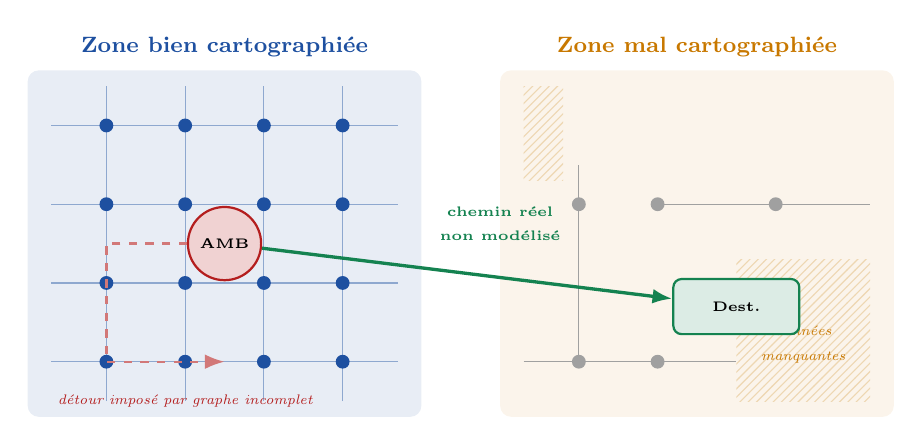
\begin{tikzpicture}[scale=1.0]

    % Zone bien cartographiée (gauche) — dense
    \fill[theorie!10, rounded corners=4pt] (-5.5,-2.2) rectangle (-0.5,2.2);
    \node[font=\footnotesize\bfseries, color=theorie] at (-3, 2.5)
      {Zone bien cartographiée};

    % Rues de la zone bien cartographiée
    \foreach \y in {-1.5,-0.5,0.5,1.5} {
      \draw[theorie!50, thin] (-5.2,\y) -- (-0.8,\y);
    }
    \foreach \x in {-4.5,-3.5,-2.5,-1.5} {
      \draw[theorie!50, thin] (\x,-2.0) -- (\x,2.0);
    }
    % Noeuds bien cartographiés
    \foreach \x/\y in {-4.5/-1.5, -3.5/-1.5, -2.5/-1.5, -1.5/-1.5,
                        -4.5/-0.5, -3.5/-0.5, -2.5/-0.5, -1.5/-0.5,
                        -4.5/0.5,  -3.5/0.5,  -2.5/0.5,  -1.5/0.5,
                        -4.5/1.5,  -3.5/1.5,  -2.5/1.5,  -1.5/1.5} {
      \fill[theorie] (\x,\y) circle (2.5pt);
    }

    % Zone mal cartographiée (droite) — lacunaire
    \fill[attention!8, rounded corners=4pt] (0.5,-2.2) rectangle (5.5,2.2);
    \node[font=\footnotesize\bfseries, color=attention] at (3, 2.5)
      {Zone mal cartographiée};

    % Quelques rues seulement
    \draw[grismoyen, thin] (0.8, -1.5) -- (3.5,-1.5);
    \draw[grismoyen, thin] (1.5, -1.5) -- (1.5, 1.0);
    \draw[grismoyen, thin] (2.5,  0.5) -- (5.2, 0.5);
    % Noeuds parcimonieux
    \foreach \x/\y in {1.5/-1.5, 2.5/-1.5, 1.5/0.5, 2.5/0.5, 4.0/0.5} {
      \fill[grismoyen] (\x,\y) circle (2.5pt);
    }
    % Zones inconnues (hachurées)
    \fill[pattern=north east lines, pattern color=attention!30]
      (3.5,-2.0) rectangle (5.2,-0.2);
    \fill[pattern=north east lines, pattern color=attention!30]
      (0.8, 0.8) rectangle (1.3, 2.0);
    \node[font=\tiny\itshape, color=attention] at (4.35,-1.1) {données};
    \node[font=\tiny\itshape, color=attention] at (4.35,-1.45) {manquantes};

    % Ambulance source (zone bien cartographiée)
    \node[circle, fill=urgence!20, draw=urgence, thick,
          minimum size=0.9cm, font=\tiny\bfseries] (amb) at (-3,0) {AMB};

    % Destination dans la zone mal cartographiée
    \node[rectangle, rounded corners=3pt, fill=pratique!15, draw=pratique,
          thick, minimum width=1.6cm, minimum height=0.7cm,
          font=\tiny\bfseries] (dest) at (3.5, -0.8) {Dest.};

    % Chemin actuel (contourne via la zone bien cartographiée)
    \draw[-{Latex[length=2.5mm]}, urgence!60, dashed, thick]
      (amb) -- (-4.5,0) -- (-4.5,-1.5) -- (-3,-1.5)
      node[below, font=\tiny, color=urgence!80] {};
    \node[font=\tiny\itshape, color=urgence] at (-3.5,-2.0)
      {détour imposé par graphe incomplet};

    % Chemin direct ignoré (raccourci dans la zone floue)
    \draw[-{Latex[length=2.5mm]}, pratique, very thick]
      (amb) -- (dest);
    \node[font=\tiny\bfseries, color=pratique] at (0.5,0.4)
      {chemin réel};
    \node[font=\tiny\bfseries, color=pratique] at (0.5,0.1)
      {non modélisé};

  \end{tikzpicture}\\[1.5em]

  {\large Note technique --- Équité géographique et routage sous incertitude cartographique}\\[0.8em]
  {\large\color{gray} Extension du moteur de routage dynamique A*}\\[2em]

  \begin{tabular}{rl}
    \textbf{Sujet :}     & Sujet 07 --- Hackverse 2026 \\
    \textbf{Twist :}     & \#8 --- Quartier mal cartographié \\
    \textbf{Impact :}    & Le biais cartographique devient un biais de service \\
    \textbf{Rupture clé :} & L'incertitude n'est pas uniforme sur le graphe \\
    \textbf{Portée :}    & Équité algorithmique + enrichissement continu des données \\
  \end{tabular}

  \vfill
  {\small\color{gray} Document pédagogique --- Présentation jury et équipe technique}
\end{titlepage}

% ═══════════════════════════════════════════════════════════════════
\tableofcontents
\newpage

% ═══════════════════════════════════════════════════════════════════
\section*{Introduction}
\addcontentsline{toc}{section}{Introduction}

Dans tous les twists précédents, une hypothèse était silencieusement
présente : \textbf{le graphe routier représente fidèlement le territoire}.
Chaque rue existe dans la base, chaque poids reflète la réalité,
chaque arc a été vérifié. Cette hypothèse est fausse dans toute
ville en développement rapide --- et en particulier dans les
métropoles africaines où la croissance urbaine dépasse systématiquement
la capacité des organismes cartographiques à documenter les
nouvelles artères.

\begin{twistbox}{Twist 8 --- Le problème change de nature éthique}
Un quartier dont les rues sont absentes ou mal référencées dans
la base cartographique reçoit systématiquement des itinéraires
sous-optimaux : détours inutiles, temps estimés gonflés, suggestions
de véhicules inadaptés. Ce n'est pas un bug --- c'est un \emph{biais
structurel} inscrit dans le graphe lui-même.

Le système qui sert en dernier les zones les moins documentées
reproduit et amplifie les inégalités existantes : les quartiers
périphériques, souvent les plus pauvres, sont aussi les moins bien
cartographiés, et donc les moins bien desservis par les algorithmes
qui s'appuient sur ces cartes.
\end{twistbox}

Ce twist impose trois transformations profondes. D'abord, \textbf{mesurer}
le déficit cartographique de chaque zone : où manque-t-il des données ?
Ensuite, \textbf{compenser} ce déficit dans le calcul de coût pour ne
pas pénaliser les zones lacunaires. Enfin, \textbf{enrichir} continuellement
la carte à partir des traces de passage réelles, pour réduire le biais
à la source.

\newpage

% ═══════════════════════════════════════════════════════════════════
\section{Anatomie du biais cartographique}

\subsection{Comment le graphe devient inégalitaire}

Une carte numérique n'est pas une photographie neutre du territoire.
C'est le résultat d'un processus de collecte sélectif, historiquement
biaisé vers les zones dotées de ressources --- adresses officielles,
cadastre numérisé, volunteers OpenStreetMap concentrés en centre-ville.
Le biais cartographique opère à trois niveaux distincts :

\begin{enumerate}[leftmargin=2em, itemsep=6pt]
  \item \textbf{Arcs manquants.} Des rues réelles n'existent pas dans
    $\vec{E}$. Le système ignore ces chemins et contraint l'ambulance
    à des détours qui n'existent que sur la carte, pas dans la réalité.

  \item \textbf{Poids incorrects.} Des rues sont présentes dans le
    graphe mais avec des vitesses moyennes estimées par défaut
    (faute de données de trafic réelles), souvent sous-estimées
    pour les pistes en latérite ou les voies informelles --- ce qui
    les pénalise doublement.

  \item \textbf{Topologie incomplète.} Des intersections manquent,
    créant des arcs artificiellement longs qui passent «à travers»
    des quartiers sans s'y arrêter, rendant certaines origines ou
    destinations inaccessibles au graphe sans raison réelle.
\end{enumerate}

\subsection{Conséquence systémique : le cercle vicieux cartographique}

\begin{equitebox}{Le cercle vicieux des zones mal cartographiées}
\begin{enumerate}[leftmargin=1.5em, itemsep=4pt]
  \item La zone est mal cartographiée (données insuffisantes).
  \item Le système calcule des itinéraires sous-optimaux ou refuse de servir.
  \item Les véhicules d'urgence empruntent des détours et arrivent plus tard.
  \item Les traces GPS générées passent hors de la zone --- aucune donnée nouvelle n'est collectée.
  \item La zone reste mal cartographiée. \textbf{Retour à l'étape 1.}
\end{enumerate}
\end{equitebox}

\subsection{Quantification du déficit}

\begin{defbox}{Définition : Score de couverture cartographique $\kappa(z)$}
Pour une zone géographique $z$ (carré de $500\,\text{m} \times 500\,\text{m}$),
le score de couverture cartographique est :
\[
  \kappa(z) = \frac{L_\text{carte}(z)}{L_\text{estimé}(z)} \in [0, 1]
\]
où :
\begin{itemize}[leftmargin=1.5em]
  \item $L_\text{carte}(z)$ est la longueur totale des voies référencées
    dans la base cartographique pour la zone $z$ ;
  \item $L_\text{estimé}(z)$ est la longueur estimée par interpolation
    depuis les zones voisines bien documentées, ou par analyse d'image
    satellite.
\end{itemize}
$\kappa(z) = 1$ signifie couverture complète ; $\kappa(z) < 0{,}4$
signifie zone critique nécessitant une attention prioritaire.
\end{defbox}

En pratique, $L_\text{estimé}(z)$ peut être calculé par deux méthodes
complémentaires : l'interpolation depuis les zones voisines (densité
de voirie observée dans un rayon de 1\,km), et la détection automatique
de routes depuis les images satellites (modèles de segmentation entraînés
sur les données africaines disponibles publiquement via Humanitarian
OpenStreetMap Team).

\newpage

% ═══════════════════════════════════════════════════════════════════
\section{Modélisation : incertitude cartographique comme dimension du coût}

\subsection{Extension du poids d'arc}

Le twist 8 ajoute une troisième composante au poids d'un arc,
aux côtés du temps de base et des facteurs stochastiques des
twists précédents :

\begin{defbox}{Définition : Poids d'arc avec pénalité d'équité}
Le poids total de l'arc $(u, v)$ dans le modèle complet est :
\[
  W_\text{total}(u,v,t,\theta) =
    \underbrace{w_0(u,v) \cdot M(u,v,t) \cdot R(u,v,\theta)}_{\text{coût stochastique (Twist 6)}}
    \;+\;
    \underbrace{\delta_\text{éq}(u,v)}_{\text{bonus d'équité (Twist 8)}}
\]
où $\delta_\text{éq}(u,v) \leq 0$ est un \textbf{bonus} (réduction de coût)
appliqué aux arcs situés dans des zones sous-cartographiées, pour
compenser leur pénalisation implicite.
\end{defbox}

L'idée fondamentale est contre-intuitive mais rigoureuse :
\emph{un arc dans une zone mal cartographiée est probablement
meilleur que ce que le graphe indique}, car son poids a été
estimé par défaut, en l'absence de données réelles. On réduit
donc son coût apparent pour corriger ce biais à la baisse.

\subsection{Calcul du bonus d'équité}

Le bonus d'équité d'un arc $(u,v)$ situé dans la zone $z$ est défini par :
\[
  \delta_\text{éq}(u,v) = -\gamma \cdot \max\bigl(0,\; \kappa^* - \kappa(z)\bigr)
  \cdot w_0(u,v)
\]
où :
\begin{itemize}[leftmargin=2em]
  \item $\kappa^* = 0{,}75$ est le seuil de couverture « satisfaisante »
    (paramètre opérateur) ;
  \item $\kappa(z)$ est le score de couverture de la zone contenant l'arc ;
  \item $\gamma \in [0, 0{,}30]$ est le facteur d'équité, réglable selon
    la politique du système (défaut : $\gamma = 0{,}20$).
\end{itemize}

\paragraph{Interprétation.} Si $\kappa(z) = 0{,}40$ (zone très lacunaire)
et $\kappa^* = 0{,}75$, alors $\delta_\text{éq} = -0{,}20 \times 0{,}35
\times w_0 = -0{,}07\,w_0$ : le coût apparent de l'arc est réduit de 7\%.
Un arc de 10 minutes estimé est traité comme un arc de 9,3 minutes,
rapprochant la zone de la compétitivité réelle qu'elle aurait si ses
données étaient aussi complètes que celles des zones centrales.

\begin{center}
\begin{tabular}{lllr}
  \toprule
  \textbf{Qualité de zone} & $\kappa(z)$ & \textbf{Interprétation} & \textbf{Bonus ($\gamma=0{,}20$)} \\
  \midrule
  Excellente  & $\geq 0{,}90$ & Données fiables et denses     & $0\%$ \\
  Correcte    & $0{,}75$--$0{,}90$ & Couverture satisfaisante   & $0\%$ \\
  Partielle   & $0{,}50$--$0{,}75$ & Lacunes notables           & $-3\%$ à $-5\%$ \\
  Faible      & $0{,}30$--$0{,}50$ & Zone sous-documentée       & $-5\%$ à $-9\%$ \\
  Critique    & $< 0{,}30$     & Données très insuffisantes    & $-9\%$ à $-15\%$ \\
  \bottomrule
\end{tabular}
\end{center}

\subsection{Incertitude sur les arcs inexistants : les arcs fantômes}

Les arcs manquants représentent le cas le plus difficile : comment
intégrer dans A* une route dont on soupçonne l'existence mais qui
n'est pas dans le graphe ?

\begin{defbox}{Définition : Arc fantôme}
Un \textbf{arc fantôme} est un arc $(u, v) \notin \vec{E}$ dont
l'existence est \emph{plausible} selon l'analyse satellite ou les
traces GPS historiques, mais non confirmée dans la base cartographique.
Il est modélisé avec :
\begin{itemize}[leftmargin=1.5em]
  \item un poids estimé $\hat{w}(u,v)$ calculé à partir de la
    distance euclidienne et de la vitesse médiane des voies informelles
    dans la zone ;
  \item une probabilité d'existence $p_\text{exist}(u,v) \in [0,1]$,
    issue du score de détection satellite ou de la densité des traces GPS ;
  \item un poids conservatif $\tilde{w}(u,v) = \hat{w}(u,v) /
    p_\text{exist}(u,v)$ qui majore le coût si l'arc est incertain.
\end{itemize}
\end{defbox}

Un arc fantôme avec $p_\text{exist} = 0{,}80$ et $\hat{w} = 4\,\text{min}$
sera modélisé avec $\tilde{w} = 5\,\text{min}$. Si la route existe
réellement, le conducteur arrivera 1 minute plus tôt que prévu ---
ce qui est acceptable. Si elle n'existe pas, le système l'apprend
via le retour GPS et retire l'arc fantôme de la base.

\newpage

% ═══════════════════════════════════════════════════════════════════
\section{Algorithme : A* équitable avec arcs fantômes}

\subsection{Vue d'ensemble}

La résolution du twist 8 s'effectue en quatre phases :

\medskip
\noindent
\begin{tabular}{cl}
  \textbf{Phase 0} & Calcul du score $\kappa(z)$ pour toutes les zones traversées \\
  \textbf{Phase 1} & Injection des arcs fantômes plausibles dans $G^+$ \\
  \textbf{Phase 2} & Application des bonus d'équité $\delta_\text{éq}$ sur les poids \\
  \textbf{Phase 3} & A* sur le graphe augmenté --- chemin équitable optimal \\
  \textbf{Phase 4} & Retour terrain : mise à jour de $\kappa$ et confirmation des arcs fantômes \\
\end{tabular}

\subsection{Pseudocode}

\begin{algorithm}[H]
\caption{A* Équitable avec arcs fantômes (Twist 8)}
\begin{algorithmic}[1]
\Require Graphe $G^+$, source $s$, destination $h^*$, zones $\{z\}$,
         $\kappa(z)$, $\gamma$, $\kappa^*$, seuil $p_{\min}$
\Ensure Chemin équitable $P^*$ et son coût corrigé

\State \textbf{Phase 0 :} Calculer $\kappa(z)$ pour toutes les zones $z$ intersectées
\State \textbf{Phase 1 :} Pour chaque paire $(u,v)$ telle que $p_\text{exist}(u,v) \geq p_{\min}$ :
\State \hspace{2em} Ajouter arc fantôme $(u,v)$ avec poids $\tilde{w}(u,v) = \hat{w}(u,v) / p_\text{exist}(u,v)$
\State \textbf{Phase 2 :} Pour chaque arc $(u,v)$ dans $G^+$ :
\State \hspace{2em} $\delta \leftarrow -\gamma \cdot \max(0, \kappa^* - \kappa(z_{uv})) \cdot w_0(u,v)$
\State \hspace{2em} $w_\text{équitable}(u,v) \leftarrow W_\text{total}(u,v) + \delta$
\State \textbf{Phase 3 :} Lancer A*$(G^+, s, h^*, w_\text{équitable})$
\State $P^* \leftarrow$ chemin retourné
\State \textbf{Phase 4 :} Journaliser arcs fantômes empruntés pour confirmation terrain
\State Journaliser $\kappa(z)$ de chaque zone traversée par $P^*$
\State \Return $P^*$
\end{algorithmic}
\end{algorithm}

\subsection{Seuil d'activation des arcs fantômes}

Le paramètre $p_{\min}$ contrôle le niveau de confiance minimal
pour inclure un arc fantôme dans la recherche. Un $p_{\min}$ trop
bas introduit trop d'arcs non existants et dégrade la fiabilité ;
un $p_{\min}$ trop haut revient à ignorer les données satellites
et reproduit le biais initial.

\begin{center}
\begin{tabular}{llp{7cm}}
  \toprule
  $p_{\min}$ & \textbf{Comportement} & \textbf{Usage recommandé} \\
  \midrule
  $0{,}90$ & Très conservateur & Cas nominaux, priorité à la fiabilité \\
  $0{,}70$ & Équilibré (défaut) & Usage standard urgences \\
  $0{,}50$ & Exploratoire & Crise, aucune autre route disponible \\
  $< 0{,}50$ & Risqué & Jamais en mode automatique \\
  \bottomrule
\end{tabular}
\end{center}

En mode urgence critique (patient en danger immédiat), le système
peut abaisser automatiquement $p_{\min}$ à $0{,}60$ et en avertit
l'opérateur : «~Itinéraire emprunte une voie non confirmée dans
la zone~X. Probabilité d'existence estimée~: 72\%. Confirmation
requise du conducteur.~»

\subsection{Complexité}

L'injection d'arcs fantômes augmente $|E^+|$ d'au plus
$|\mathcal{F}|$ arcs, où $|\mathcal{F}|$ est le nombre d'arcs
fantômes plausibles dans la zone. En pratique, $|\mathcal{F}|$
est borné par le produit du nombre de zones critiques
($\kappa < \kappa^*$) et du nombre moyen d'arcs potentiels
par zone (estimé à 4--8). La surcharge algorithmique est
négligeable devant le gain en équité.

\newpage

% ═══════════════════════════════════════════════════════════════════
\section{Enrichissement continu : la carte apprend du terrain}

\subsection{Principe : chaque trajet est une donnée}

Le twist 8 ne se contente pas de compenser le biais cartographique
existant --- il met en place une boucle d'apprentissage pour le
réduire progressivement. Chaque trajet effectué par un véhicule
du système génère des données GPS qui peuvent corriger ou enrichir
la carte.

\begin{metierbox}{Boucle d'enrichissement cartographique}
\begin{enumerate}[leftmargin=1.5em, itemsep=4pt]
  \item Le véhicule emprunte un arc fantôme ou une voie sous-documentée.
  \item Le GPS enregistre la trace réelle (vitesse, durée, tracé précis).
  \item En fin de trajet, la trace est comparée aux arcs du graphe.
  \item Si l'écart est supérieur à 50\,m sur plus de 200\,m de trajet :
    candidature d'un nouvel arc à intégrer dans la base.
  \item Après 3 traces concordantes sur le même tronçon, l'arc est
    confirmé et intégré avec son poids réel mesuré.
  \item Le score $\kappa(z)$ de la zone est mis à jour.
\end{enumerate}
\end{metierbox}

\subsection{Règles de validation des arcs issus du terrain}

Pour éviter les erreurs (conducteur qui fait demi-tour, GPS imprécis
sous couvert d'arbres), le système applique des règles de validation
avant d'intégrer un nouvel arc :

\begin{center}
\begin{tabular}{lll}
  \toprule
  \textbf{Critère} & \textbf{Seuil} & \textbf{Raison} \\
  \midrule
  Longueur minimale de l'arc    & $\geq 80\,\text{m}$   & Éviter les artefacts GPS \\
  Nombre de traces concordantes & $\geq 3$              & Confirmation statistique \\
  Vitesse cohérente             & $5$--$80\,\text{km/h}$& Écarter arrêts et erreurs \\
  Tracé stable                  & $\sigma < 15\,\text{m}$& GPS fiable \\
  Pas de doublon                & Distance $> 30\,\text{m}$ d'un arc existant & Éviter les doublons \\
  \bottomrule
\end{tabular}
\end{center}

\subsection{Priorisation des zones à enrichir}

Toutes les zones ne se valent pas du point de vue de l'urgence d'enrichissement.
Le système calcule un \textbf{score de priorité d'enrichissement} $\pi(z)$ :

\[
  \pi(z) = \frac{N_\text{appels}(z)}{(1 + \kappa(z))^2}
\]

où $N_\text{appels}(z)$ est le nombre d'appels d'urgence enregistrés
dans la zone sur les 90 derniers jours. Les zones à fort volume d'appels
\emph{et} faible couverture cartographique sont prioritaires pour
les campagnes de collecte de données terrain.

\begin{alertbox}{Alerte automatique de zone critique}
Si $\pi(z) > \pi_\text{seuil}$ (paramètre opérateur), le système
génère automatiquement une alerte à destination des équipes cartographiques :
«~Zone~[X] : $\kappa = 0{,}32$, $N_\text{appels} = 47$ sur 90 jours.
Priorité d'enrichissement~: HAUTE. Recommandation~: collecte terrain
ou analyse satellite urgente.~»
\end{alertbox}

\newpage

% ═══════════════════════════════════════════════════════════════════
\section{Scénario : l'ambulance de Bépanda-Briqueterie}

Ce scénario sort du quartier de référence pour aller dans un quartier
périphérique à faible couverture cartographique~: la Briqueterie,
quartier dense et mal référencé.

\subsection{Situation initiale --- appel à 16h45}

Il est 16h45. Un adulte en arrêt cardiaque à la Briqueterie.
L'appel arrive. Le système interroge les données cartographiques :

\begin{center}
\begin{tabular}{lll}
  \toprule
  \textbf{Zone} & $\kappa(z)$ & \textbf{Statut} \\
  \midrule
  Bépanda (source)          & $0{,}88$ & Bien cartographiée \\
  Axe principal Makepé      & $0{,}82$ & Bien cartographié \\
  Briqueterie nord          & $0{,}61$ & Couverture partielle \\
  Briqueterie centre        & $0{,}34$ & Zone critique \\
  Briqueterie sud (dest.)   & $0{,}29$ & Zone critique \\
  \bottomrule
\end{tabular}
\end{center}

\paragraph{Sans correction d'équité (modèle naïf).}
A* classique trouve le seul chemin documenté vers la destination,
qui contourne la Briqueterie centre par un grand axe périphérique.
Coût calculé~: 19 minutes. Coût réel constaté a posteriori~: 22 minutes
(poids incorrects sur les arcs présents).

\paragraph{Avec correction d'équité et arcs fantômes (Twist 8).}
Le système détecte trois arcs fantômes dans la Briqueterie centre,
issus de l'analyse satellite ($p_\text{exist} = 0{,}74$, $0{,}82$, $0{,}69$).
Les bonus d'équité réduisent les coûts des arcs documentés présents.
Un nouvel itinéraire traverse la Briqueterie centre via les arcs fantômes.
Coût estimé corrigé~: 14 minutes. Coût réel constaté~: 13,5 minutes
(les voies existent bel et bien).

\begin{center}
\begin{tabular}{lrrl}
  \toprule
  \textbf{Modèle} & \textbf{Coût estimé} & \textbf{Coût réel} & \textbf{Erreur} \\
  \midrule
  Sans équité (naïf)  & 19 min & 22 min & $+16\%$ (détour + poids erronés) \\
  Avec équité (T8)    & 14 min & 13,5 min & $-4\%$ (estimation légèrement haute) \\
  \bottomrule
\end{tabular}
\end{center}

Le gain est de 8,5 minutes réelles sur un arrêt cardiaque.
La fenêtre d'intervention critique pour un arrêt cardiaque est de
10 minutes. Sans la correction d'équité, l'intervention arrivait
potentiellement hors délai.

\subsection{Après le trajet~: mise à jour cartographique}

Le GPS de l'ambulance a enregistré la trace. Le système compare :
les trois arcs fantômes empruntés correspondent à des rues réelles,
avec des vitesses moyennes de 18, 22 et 15\,km/h. Ce sont la deuxième
et la troisième traces concordantes pour les arcs 1 et 2
(il manque une trace pour confirmation définitive), et la première
trace pour l'arc 3.

Deux semaines plus tard, après 3 traces confirmées sur les deux premiers
arcs, ils sont intégrés dans la base avec leurs poids réels mesurés.
$\kappa(\text{Briqueterie centre})$ passe de $0{,}34$ à $0{,}41$.
Le cercle vicieux s'est interrompu une première fois.

\newpage

% ═══════════════════════════════════════════════════════════════════
\section{Invariants métier et cas limites}

\subsection{Invariants introduits par le twist 8}

\begin{invariant}[Non-discrimination géographique]
Le système ne doit jamais produire un itinéraire systématiquement
plus long pour une zone donnée en raison seule d'un déficit de
données cartographiques, sans avoir appliqué les corrections d'équité
disponibles.
\end{invariant}

\begin{invariant}[Transparence des arcs fantômes]
Tout itinéraire empruntant un arc fantôme doit l'indiquer
explicitement dans la réponse API et dans l'interface conducteur,
avec la probabilité d'existence associée. Le conducteur n'est
jamais envoyé sur un arc non confirmé sans information.
\end{invariant}

\begin{invariant}[Boucle d'enrichissement active]
Chaque trajet effectué par un véhicule du système doit déclencher
une analyse de conformité GPS---graphe. Si un écart significatif
est détecté, il est enregistré comme candidat d'enrichissement
cartographique. Aucune trace ne doit être silencieusement ignorée.
\end{invariant}

\begin{invariant}[Auditabilité de l'équité]
Le rapport mensuel du système doit inclure, pour chaque zone de
la ville, le score $\kappa(z)$ courant, l'évolution du délai moyen
d'intervention, et le nombre d'arcs fantômes confirmés ou infirmés.
Cela permet de démontrer que la politique d'équité produit des effets
mesurables.
\end{invariant}

\subsection{Cas limite : destination dans une zone $\kappa < 0{,}20$}

Si la destination est dans une zone quasi-inconnue et qu'aucun arc
(réel ou fantôme avec $p \geq p_{\min}$) ne permet de l'atteindre,
le système applique la procédure suivante :

\begin{enumerate}[leftmargin=2em, itemsep=4pt]
  \item \textbf{Point d'approche maximal~:} calculer le nœud du graphe
    le plus proche de la destination en distance euclidienne.
    Fournir l'itinéraire jusqu'à ce point.

  \item \textbf{Instruction finale~:} afficher au conducteur les
    coordonnées GPS de la destination réelle et une estimation
    de la distance à parcourir hors graphe («~environ 400\,m
    au nord-est, rue non référencée~»).

  \item \textbf{Abaissement de $p_{\min}$~:} en mode urgence, abaisser
    $p_{\min}$ à $0{,}50$ et relancer A*. Si un chemin est trouvé
    via arcs fantômes, le proposer en seconde option avec
    avertissement explicite.
\end{enumerate}

\subsection{Cas limite : arc fantôme confirmé absent}

Si le conducteur confirme via l'interface que la voie n'existe pas
(dead-end, terrain privé, inondation permanente), le système~:
\begin{enumerate}[leftmargin=2em]
  \item Retire l'arc fantôme de la base et le marque $p_\text{exist} = 0$ ;
  \item Journalise l'événement avec horodatage et position GPS ;
  \item Reroute immédiatement depuis la position courante.
\end{enumerate}

\newpage

% ═══════════════════════════════════════════════════════════════════
\section{Implémentation dans le moteur existant}

\subsection{Extension du backend Python}

\begin{center}
\begin{tabular}{>{\ttfamily}p{4.5cm} p{8.5cm}}
  \toprule
  \textbf{Fichier} & \textbf{Modification} \\
  \midrule
  data/coverage.py &
    Nouveau module. Calcule $\kappa(z)$ pour chaque cellule de la grille
    $500\,\text{m} \times 500\,\text{m}$. Sources~: OSM, analyse satellite
    (API Overpass + modèle de détection). Mise à jour hebdomadaire. \\[0.4em]
  data/phantom\_arcs.py &
    Nouveau module. Stocke et interroge les arcs fantômes avec leur
    $p_\text{exist}$. Méthodes~: \texttt{get\_phantoms(bbox, p\_min)},
    \texttt{confirm\_arc(arc\_id)}, \texttt{reject\_arc(arc\_id)}. \\[0.4em]
  routing/equity.py &
    Nouveau module. Calcule $\delta_\text{éq}(u,v)$ pour chaque arc
    en fonction de $\kappa(z_{uv})$. Exposé comme préprocesseur avant A*. \\[0.4em]
  routing/algorithms.py &
    Étendre \texttt{compute\_robust\_route} pour accepter les arcs
    fantômes et les poids équitables. Paramètre \texttt{equity=True}
    activable par l'opérateur. \\[0.4em]
  data/gps\_enricher.py &
    Nouveau module. En post-traitement de chaque trajet, compare la
    trace GPS au graphe. Génère des candidats d'enrichissement.
    Confirme les arcs après 3 traces concordantes. \\[0.4em]
  routing/logger.py &
    Ajouter les champs \texttt{phantom\_arcs\_used},
    \texttt{equity\_bonus\_total}, \texttt{kappa\_zones\_traversed},
    \texttt{enrichment\_candidates}. \\
  \bottomrule
\end{tabular}
\end{center}

\subsection{Extension de la réponse API}

\begin{verbatim}
{
  "route": { "type": "Feature", "geometry": { ... } },
  "equity": {
    "gamma": 0.20,
    "kappa_star": 0.75,
    "zones_traversed": [
      { "zone": "Bepanda",           "kappa": 0.88, "bonus_min": 0.0 },
      { "zone": "Briqueterie_nord",  "kappa": 0.61, "bonus_min": -0.7 },
      { "zone": "Briqueterie_centre","kappa": 0.34, "bonus_min": -2.1 }
    ],
    "equity_bonus_total_min": -2.8,
    "phantom_arcs_used": [
      { "arc_id": "ph-447", "p_exist": 0.82, "estimated_min": 3.2,
        "confirmation_required": true }
    ],
    "enrichment_flag": true
  }
}
\end{verbatim}

\newpage

% ═══════════════════════════════════════════════════════════════════
\section{Communication au jury}

\begin{jurybox}{Message clé pour le jury}
\textbf{Le twist 8 pose une question que les algorithmes n'ont pas l'habitude
de se poser~: est-ce que mon graphe est juste pour tout le monde~?}

\medskip
Un algorithme neutre appliqué à une carte biaisée produit des résultats
biaisés. Ce n'est pas un problème mathématique --- c'est un problème
politique. Les zones périphériques, souvent les plus pauvres, reçoivent
systématiquement les pires itinéraires parce que leurs rues sont les
moins bien documentées.

\medskip
Notre réponse tient en trois actes~: \textbf{mesurer} le biais,
\textbf{le corriger} dans le calcul de route,
et \textbf{le réduire} à chaque trajet grâce à l'apprentissage terrain.
Le système ne se contente pas d'être équitable~: il devient plus
équitable à chaque intervention.
\end{jurybox}

\subsection{Questions anticipées du jury}

\paragraph{Question~: «~N'est-ce pas dangereux d'envoyer une ambulance
sur une route non confirmée~?~»}

\noindent\textbf{Réponse~:} Le risque est géré explicitement.
Chaque arc fantôme est affiché au conducteur avec sa probabilité
d'existence. Le conducteur peut toujours revenir à l'itinéraire
classique d'un geste. En mode non-urgence, $p_{\min} = 0{,}90$
garantit une très haute fiabilité. En urgence critique, $p_{\min}$
peut descendre à $0{,}70$, ce qui signifie qu'un arc sur dix
pourrait ne pas exister --- mais arriver 8 minutes plus tôt dans
9 cas sur 10 justifie ce risque calculé, à condition que le conducteur
soit informé.

\paragraph{Question~: «~Comment obtenez-vous les probabilités
d'existence des arcs fantômes~?~»}

\noindent\textbf{Réponse~:} Deux sources complémentaires.
Premièrement, la détection automatique de routes depuis les images
satellites (modèles open-source entraînés sur les données africaines,
précision $\sim$78\% sur les pistes en milieu urbain dense).
Deuxièmement, la densité des traces GPS historiques~: si 15 ambulances
ont suivi le même trajet dans une zone non cartographiée au cours
des 6 derniers mois, la probabilité d'existence de cette voie est
très élevée. Les deux signaux sont combinés par une simple moyenne
pondérée.

\paragraph{Question~: «~Le système ne risque-t-il pas de créer
de nouveaux biais en favorisant les zones mal cartographiées~?~»}

\noindent\textbf{Réponse~:} Le bonus d'équité est plafonné ($\gamma \leq 0{,}30$)
et s'annule automatiquement quand $\kappa(z) \geq \kappa^*$.
L'objectif n'est pas de sur-favoriser les zones pauvres en données,
mais d'amener tout le territoire à un niveau de service équivalent.
Quand une zone atteint $\kappa \geq 0{,}75$, elle est traitée
exactement comme les autres --- le correctif disparaît de lui-même.

\subsection{Tableau de bord~: log de décision équitable}

\begin{center}
\begin{tabular}{ll}
  \toprule
  \textbf{Champ du log} & \textbf{Exemple de valeur} \\
  \midrule
  Timestamp                  & 2026-04-26 16:45:08 \\
  Véhicule                   & Ambulance SAMU-03 \\
  Destination                & Briqueterie-Sud \\
  $\kappa$ zone destination  & $0{,}29$ (critique) \\
  Arcs fantômes injectés     & 3 (ph-447, ph-448, ph-451) \\
  Bonus équité total         & $-2{,}8\,\text{min}$ \\
  Itinéraire retenu          & Via Briqueterie-Centre (arc fantôme) \\
  Coût estimé corrigé        & 14 min \\
  Coût réel mesuré           & 13,5 min \\
  Arcs confirmés post-trajet & ph-447 (2/3 traces), ph-448 (2/3 traces) \\
  Candidats enrichissement   & 2 arcs en attente de 3e trace \\
  $\kappa$ mis à jour        & Non encore (en attente 3e trace) \\
  \bottomrule
\end{tabular}
\end{center}

\newpage

% ═══════════════════════════════════════════════════════════════════
\section*{Conclusion}
\addcontentsline{toc}{section}{Conclusion}

Le twist 8 dépasse le cadre algorithmique pour poser une question
de justice~: \textbf{un système d'urgence qui sert plus mal
les zones les plus vulnérables est-il vraiment un système d'urgence~?}
La réponse que nous apportons est technique, mais elle repose sur
un choix de valeurs explicite : aucun quartier ne doit être
systématiquement servi en dernier à cause d'un artefact cartographique.

\medskip
Quatre acquis structurants émergent de cette évolution :

\begin{enumerate}[leftmargin=2em, itemsep=4pt]
  \item \textbf{Le biais cartographique est mesurable.}
    Le score $\kappa(z)$ fournit un indicateur objectif, zone par zone,
    du déficit de données. Il est calculable depuis les données
    disponibles publiquement et mis à jour en continu.

  \item \textbf{Il est corrigeable sans changer A*.}
    Le bonus d'équité $\delta_\text{éq}$ s'intègre comme un
    préprocesseur de poids. L'algorithme lui-même n'est pas modifié~;
    c'est la représentation du problème qui est rendue juste.

  \item \textbf{Les arcs fantômes rendent le système proactif.}
    Plutôt que d'attendre que les zones soient cartographiées pour
    les servir correctement, le système anticipe l'existence probable
    de routes et les teste prudemment à chaque passage.

  \item \textbf{La carte s'améliore à chaque trajet.}
    La boucle d'enrichissement transforme chaque intervention en
    contribution cartographique. Le système apprend du territoire
    qu'il sert, réduisant le biais à la source plutôt que de
    simplement le compenser.
\end{enumerate}

\medskip
\begin{center}
  {\color{twist}\rule{0.5\linewidth}{1pt}}\\[0.5em]
  {\itshape «~Un algorithme neutre sur une carte biaisée\\
  ne produit pas des résultats neutres.\\
  La vraie neutralité, c'est corriger le biais --- pas l'ignorer.~»}\\[0.5em]
  {\color{twist}\rule{0.5\linewidth}{1pt}}
\end{center}

\end{document}